% Basic LaTeX template for NE 204 lab report
\documentclass[11pt]{article}

%==============================================================================
%%% Everything between the "="'s is the preamble.
%%% Define packages and meta data here

% Common packages
\usepackage{amsmath}    % Expanded math
\usepackage{amssymb}    % Expanded math symbols
\usepackage{graphicx}   % For images
%\usepackage[version=3]{mhchem} % For nuclide formatting

% All images/figures will be stored in the images folder.
% Specify that here so pdflatex knows where to look for images.
\graphicspath{{./images/}}

% Metadata
\title{Calibration Lab report}
\author{Dajie Sun}
\date{\today}
%==============================================================================

\begin{document}

% Compile metadata from preamble into a nicely-rendered title section
\maketitle

% The *'s next so section/subsection definitions suppresses numbering
\section*{Introduction}
\label{sec:intro}
Energy calibration of a HPGe detector is an ubiquitous task in radiation detection laboratories, in this experiment, the main purpose is to practice generating lab reports using the reproducible workflow required for this course.


\section*{Methods}
\label{sec:meth}
This is not a real lab in the sense that we don't need to collect data by ourselves. The data is given by the instrutor and can be downloaded by students. Because this experiment is actually used to practice writing lab reports, so what we have to do is doing energy calibration using the data given us.

The data file consists of pulse height spectra taken with a coaxial HPGe detector using 5 different radionuclide calibration sources: 241 Am, 133 Ba,137 Cs, 60 Co, and 152 Eu. The MCA with which the data was collected had 13-bit resolution, yielding 8192 channels. As the charteristical energy of the full energy peaks of these 5 radionuclide is already known, which is to say you can find their spectrum in textbook or nuclear data website, we only need to find out the centroid of each peak and correlate it with its energy using least square method.


\[Energy=slope\cdot Channel\,Number + intercept\]

As for each full energy peak, we use gaus curve to simulate and get the centroid (B) of each peak:
\[f\left( x \right) = A \cdot {e^{ - \frac{{{{\left( {x - B} \right)}^2}}}{{2 \cdot {C^2}}}}}\]

and this is acheived by function $curve\_fit$.

Now, the centroid of each peak and its corresponding energy are known, we can make linear regression using least square method to find the relationship between the channel number and its corresponding energy value.




\section*{Results}
\label{sec:res}
Totally, we found 17 peaks and their corresponding energy, listed as the table below:

\begin{table}[h!]
  \begin{center}
    \caption{Peaks with Corresponding Energy.}
    \label{tab:table1}
    \begin{tabular}{l|l|l}
      \textbf{Peak \#} & \textbf{Channel \#} & \textbf{Energy(keV)}\\
      \hline
      1 & 207.72934164066072 & 59.5409\\
      2 & 2353.969595281511 & 661.657\\
      3 & 4177.6835240821465 & 1173.228\\
      4 & 4745.511220436352  & 1332.492\\
      5 & 429.56728236065885 & 121.7817\\
      6 & 867.77043054316  & 244.6974\\
      7 & 1222.6117121691966  & 344.2785\\
      8 & 1460.7650922753362  & 411.1165\\
      9 & 2772.003206539464  & 778.9045\\
      10 & 3432.077389155436 & 964.072\\
      11 & 5014.927456550307 & 1408.013\\
      12 & 3959.8315489345346 & 1112.076\\
      13 & 284.28923089774975 & 80.9979\\
      14 & 980.9088851006587  & 276.3989\\
      15 & 1075.1587761476976 & 302.8508\\
      16 & 1264.6138573728588 & 356.0129\\
      17 & 1363.8190002015974 & 383.8485\\
 
    \end{tabular}
  \end{center}
\end{table}
Making a linear regression of the table above, we have
\[Energy[keV]=0.280521278253 \cdot Channel\,Number+1.27621057811\,\,\,\,\,\,\,\,\,(1)\]
with the coefficient of determination ${R^2}$:
\[{R^2}=0.999999997516\]
which is very close to 1. so the calibration result is very good.




\begin{figure}
  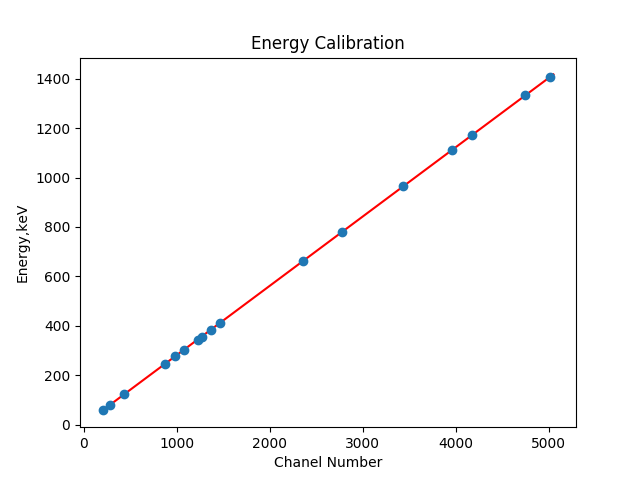
\includegraphics[scale=0.6]{Calibration}
  \caption{Energy Calibration.}
  \label{fig:boat1}
\end{figure}

\section*{Discussion}
\label{sec:disc}
If only using the peak of Am-241(59.5409 keV) and the peak of Cs-137 (661.657 keV), an approximation result is got as:
\[{Energy^*}=0.2805446 \cdot Channel\,Number+1.263557\,\,\,\,\,\,\,\,\,(2)\]

Compare Equation (1) with Equation (2), it is found they are still very close, especially with respect to the slope.


% Bibliography
\bibliographystyle{plain}
% Refers to a bibtex file in the current dir named "references.bib"
\bibliography{references}

\end{document}
